% Sources: ULXspectra-mc docs/figures/fits_by_source_mc_0p3-10keV.pdf, script docs/scripts/plot_fits_by_source.py (commit 7dd40e3; page 6 redrawn in 8176d9c);
%          included as is (author 2026-11-20). To be remade for the refit round with the 190-run table (run tag mc28_0p3-10keV).

\section{Overview of the fits}
\label{app:fitsoverview}

Figures~\ref{fig:fits_M}--\ref{fig:fits_spectra} show all fits of the round with the transfer correction over 0.3--10\,keV (run tag \code{mc\_0p3-10keV}, 13 presets for each of the 14 sources), made with the 117-run table of the correction (App.~\ref{app:mc:table}).
In Figs.~\ref{fig:fits_M}--\ref{fig:fits_rin} each source has a panel, and each preset a point: the posterior median of a parameter with its 68\% interval against the normalized reduced $\chi^2 = \chi^2/(n - k)$ of the saved best fit ($\sigma = 0.08$\,dex); BH presets are black, NS presets orange, and a parameter fixed by the preset is drawn as a horizontal dash at its value.
Figure~\ref{fig:fits_spectra} shows the model spectra of all presets.
These figures will be remade for the refits with the revised table.

\begin{figure*}[p]
\centering
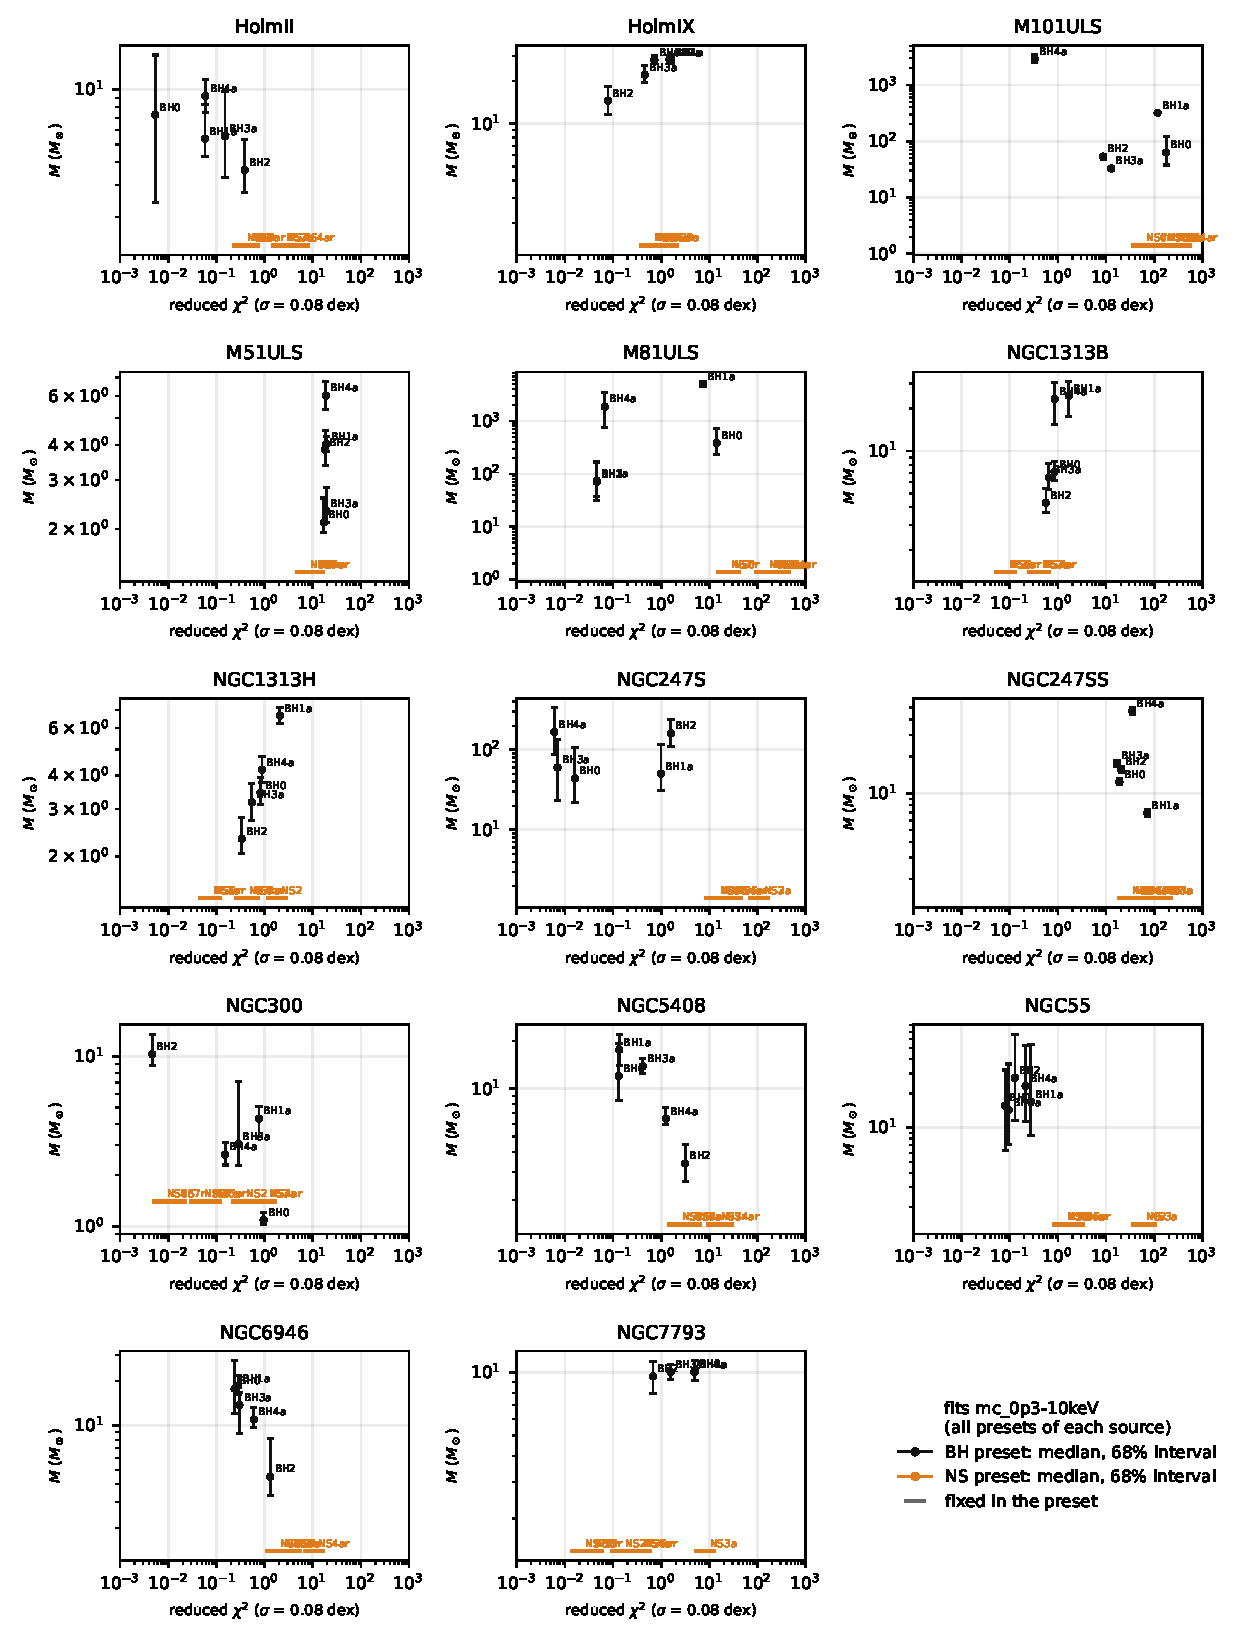
\includegraphics[page=1,width=\textwidth]{fits_by_source_mc_0p3-10keV.pdf}
\caption{All fits with the transfer correction (0.3--10\,keV, 117-run table), one panel per source: the accretor mass $M$ ($M_\odot$) against the normalized reduced $\chi^2$ of the best fit ($\sigma = 0.08$\,dex).
Points: posterior median and 68\% interval of each preset, BH black, NS orange, the preset named beside its point; dashes: values fixed by the preset.
Made with \code{docs/scripts/plot\_fits\_by\_source.py} (code commit 7dd40e3).}
\label{fig:fits_M}
\end{figure*}

\begin{figure*}[p]
\centering
\includegraphics[page=2,width=\textwidth]{fits_by_source_mc_0p3-10keV.pdf}
\caption{All fits with the transfer correction (0.3--10\,keV, 117-run table), one panel per source: the inclination $i$ (degrees) against the normalized reduced $\chi^2$ of the best fit ($\sigma = 0.08$\,dex).
Points: posterior median and 68\% interval of each preset, BH black, NS orange, the preset named beside its point; dashes: values fixed by the preset.
Made with \code{docs/scripts/plot\_fits\_by\_source.py} (code commit 7dd40e3).}
\label{fig:fits_i}
\end{figure*}

\begin{figure*}[p]
\centering
\includegraphics[page=3,width=\textwidth]{fits_by_source_mc_0p3-10keV.pdf}
\caption{All fits with the transfer correction (0.3--10\,keV, 117-run table), one panel per source: the wind toll $\epsilon_{\rm w}$ against the normalized reduced $\chi^2$ of the best fit ($\sigma = 0.08$\,dex).
Points: posterior median and 68\% interval of each preset, BH black, NS orange, the preset named beside its point; dashes: values fixed by the preset.
Made with \code{docs/scripts/plot\_fits\_by\_source.py} (code commit 7dd40e3).}
\label{fig:fits_epsw}
\end{figure*}

\begin{figure*}[p]
\centering
\includegraphics[page=4,width=\textwidth]{fits_by_source_mc_0p3-10keV.pdf}
\caption{All fits with the transfer correction (0.3--10\,keV, 117-run table), one panel per source: the inner accretion rate $\dot m_{\rm in}/\dot m_0$ (presets with a set inner rate only) against the normalized reduced $\chi^2$ of the best fit ($\sigma = 0.08$\,dex).
Points: posterior median and 68\% interval of each preset, BH black, NS orange, the preset named beside its point; dashes: values fixed by the preset.
Made with \code{docs/scripts/plot\_fits\_by\_source.py} (code commit 7dd40e3).}
\label{fig:fits_fin}
\end{figure*}

\begin{figure*}[p]
\centering
\includegraphics[page=5,width=\textwidth]{fits_by_source_mc_0p3-10keV.pdf}
\caption{All fits with the transfer correction (0.3--10\,keV, 117-run table), one panel per source: the inner disc radius $\rin/\rg$ (NS: $\rmag/\rg$) against the normalized reduced $\chi^2$ of the best fit ($\sigma = 0.08$\,dex).
Points: posterior median and 68\% interval of each preset, BH black, NS orange, the preset named beside its point; dashes: values fixed by the preset.
Made with \code{docs/scripts/plot\_fits\_by\_source.py} (code commit 7dd40e3).}
\label{fig:fits_rin}
\end{figure*}

\begin{figure*}[p]
\centering
\includegraphics[page=6,width=\textwidth]{fits_by_source_mc_0p3-10keV.pdf}
\caption{Model spectra of all fits with the transfer correction (0.3--10\,keV, 117-run table), one panel per source: the observed SED (grey line), the fitted points (dots; the fitted band shaded orange for the NS and NS candidates of Table~\ref{tab:sources}, grey for the BH candidates) and the best-fit model of every preset, BH black and grey, NS orange; the best BH and the best NS fit are drawn thicker, and their normalized reduced $\chi^2$ are given above each panel.
Made with \code{docs/scripts/plot\_fits\_by\_source.py} (code commit 8176d9c).}
\label{fig:fits_spectra}
\end{figure*}
